% PRIME Results Charts (TikZ + pgfplots)
% Include this in main.tex with: % PRIME Results Charts (TikZ + pgfplots)
% Include this in main.tex with: % PRIME Results Charts (TikZ + pgfplots)
% Include this in main.tex with: % PRIME Results Charts (TikZ + pgfplots)
% Include this in main.tex with: \input{figures/results_chart.tex}

% Embedder Comparison Bar Chart
\begin{figure}[t]
\centering
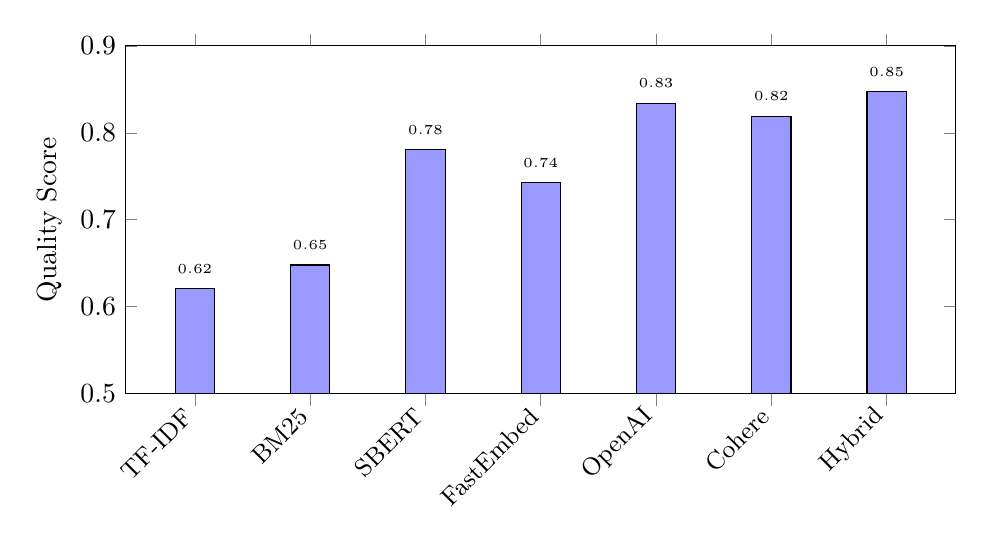
\begin{tikzpicture}
\begin{axis}[
    ybar,
    width=\columnwidth,
    height=6cm,
    ylabel={Quality Score},
    symbolic x coords={TF-IDF, BM25, SBERT, FastEmbed, OpenAI, Cohere, Hybrid},
    xtick=data,
    x tick label style={rotate=45, anchor=east, font=\small},
    ymin=0.5,
    ymax=0.9,
    bar width=0.5cm,
    nodes near coords,
    nodes near coords style={font=\tiny},
    legend style={at={(0.5,1.15)}, anchor=south, legend columns=2, font=\small},
    every node near coord/.append style={font=\tiny, yshift=2pt}
]
\addplot[fill=blue!40] coordinates {
    (TF-IDF, 0.621)
    (BM25, 0.648)
    (SBERT, 0.781)
    (FastEmbed, 0.743)
    (OpenAI, 0.834)
    (Cohere, 0.819)
    (Hybrid, 0.847)
};
\end{axis}
\end{tikzpicture}
\caption{Quality score comparison across embedding strategies. Hybrid retrieval (BM25 + SBERT) achieves the highest quality.}
\label{fig:embedder_comparison}
\end{figure}

% Generator Comparison Chart
\begin{figure}[t]
\centering
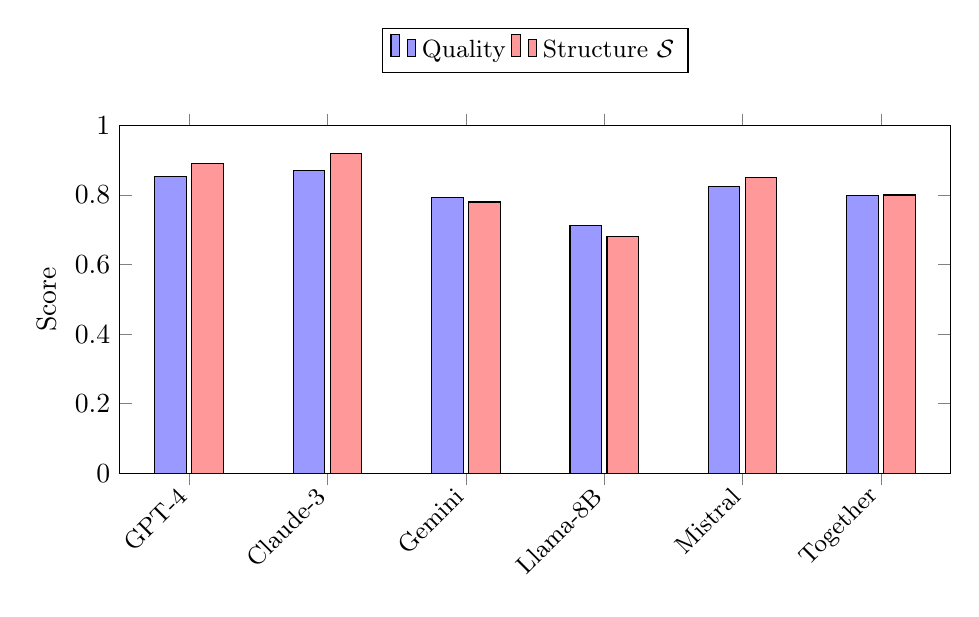
\begin{tikzpicture}
\begin{axis}[
    ybar,
    width=\columnwidth,
    height=6cm,
    ylabel={Score},
    symbolic x coords={GPT-4, Claude-3, Gemini, Llama-8B, Mistral, Together},
    xtick=data,
    x tick label style={rotate=45, anchor=east, font=\small},
    ymin=0,
    ymax=1,
    bar width=0.4cm,
    legend style={at={(0.5,1.15)}, anchor=south, legend columns=2, font=\small},
]
\addplot[fill=blue!40] coordinates {
    (GPT-4, 0.852)
    (Claude-3, 0.871)
    (Gemini, 0.793)
    (Llama-8B, 0.712)
    (Mistral, 0.824)
    (Together, 0.798)
};
\addlegendentry{Quality}
\addplot[fill=red!40] coordinates {
    (GPT-4, 0.89)
    (Claude-3, 0.92)
    (Gemini, 0.78)
    (Llama-8B, 0.68)
    (Mistral, 0.85)
    (Together, 0.80)
};
\addlegendentry{Structure $\mathcal{S}$}
\end{axis}
\end{tikzpicture}
\caption{Generator comparison showing overall quality and structural coherence scores.}
\label{fig:generator_comparison}
\end{figure}

% Quality vs Latency Scatter Plot
\begin{figure}[t]
\centering
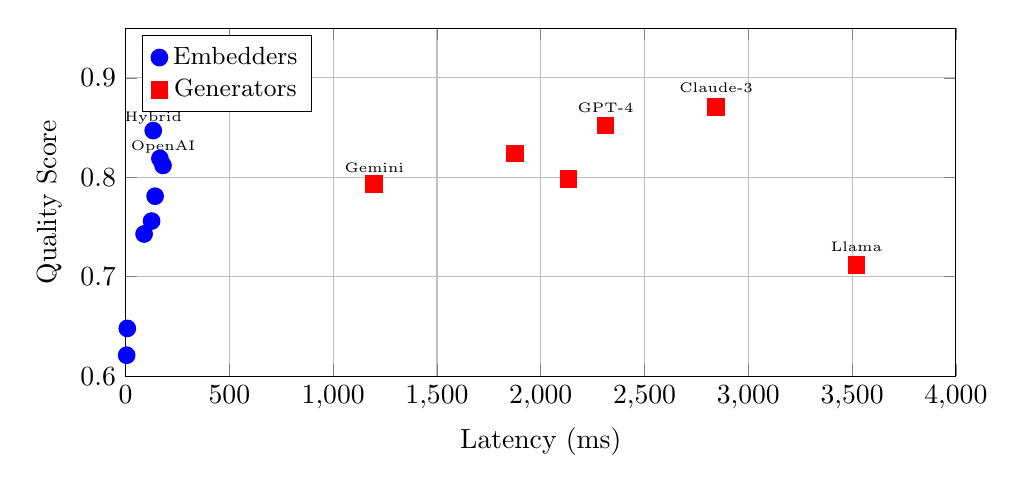
\begin{tikzpicture}
\begin{axis}[
    width=\columnwidth,
    height=6cm,
    xlabel={Latency (ms)},
    ylabel={Quality Score},
    xmin=0,
    xmax=4000,
    ymin=0.6,
    ymax=0.95,
    grid=major,
    legend style={at={(0.02,0.98)}, anchor=north west, font=\small},
]
% Embedders
\addplot[only marks, mark=*, mark size=3pt, blue] coordinates {
    (5, 0.621)
    (8, 0.648)
    (125, 0.756)
    (142, 0.781)
    (89, 0.743)
    (180, 0.812)
    (165, 0.819)
    (133, 0.847)
};
\addlegendentry{Embedders}

% Generators
\addplot[only marks, mark=square*, mark size=3pt, red] coordinates {
    (2312, 0.852)
    (2845, 0.871)
    (1198, 0.793)
    (3521, 0.712)
    (1876, 0.824)
    (2134, 0.798)
};
\addlegendentry{Generators}

% Labels
\node[font=\tiny] at (axis cs:180, 0.83) {OpenAI};
\node[font=\tiny] at (axis cs:133, 0.86) {Hybrid};
\node[font=\tiny] at (axis cs:2312, 0.87) {GPT-4};
\node[font=\tiny] at (axis cs:2845, 0.89) {Claude-3};
\node[font=\tiny] at (axis cs:1198, 0.81) {Gemini};
\node[font=\tiny] at (axis cs:3521, 0.73) {Llama};

\end{axis}
\end{tikzpicture}
\caption{Quality vs. latency tradeoff for embedders (blue circles) and generators (red squares). Gemini offers the best latency/quality ratio among generators.}
\label{fig:quality_latency}
\end{figure}

% Ablation Study Line Chart
\begin{figure}[t]
\centering
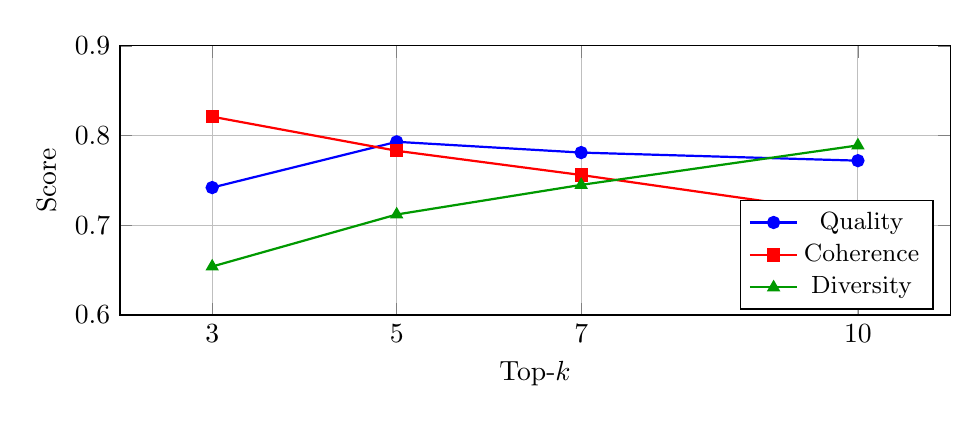
\begin{tikzpicture}
\begin{axis}[
    width=\columnwidth,
    height=5cm,
    xlabel={Top-$k$},
    ylabel={Score},
    xmin=2,
    xmax=11,
    ymin=0.6,
    ymax=0.9,
    xtick={3,5,7,10},
    legend style={at={(0.98,0.02)}, anchor=south east, font=\small},
    grid=major,
]
\addplot[blue, thick, mark=*] coordinates {
    (3, 0.742)
    (5, 0.793)
    (7, 0.781)
    (10, 0.772)
};
\addlegendentry{Quality}
\addplot[red, thick, mark=square*] coordinates {
    (3, 0.821)
    (5, 0.783)
    (7, 0.756)
    (10, 0.712)
};
\addlegendentry{Coherence}
\addplot[green!60!black, thick, mark=triangle*] coordinates {
    (3, 0.654)
    (5, 0.712)
    (7, 0.745)
    (10, 0.789)
};
\addlegendentry{Diversity}
\end{axis}
\end{tikzpicture}
\caption{Effect of top-$k$ on quality metrics. $k=5$ balances quality and coherence optimally.}
\label{fig:topk_ablation}
\end{figure}



% Embedder Comparison Bar Chart
\begin{figure}[t]
\centering
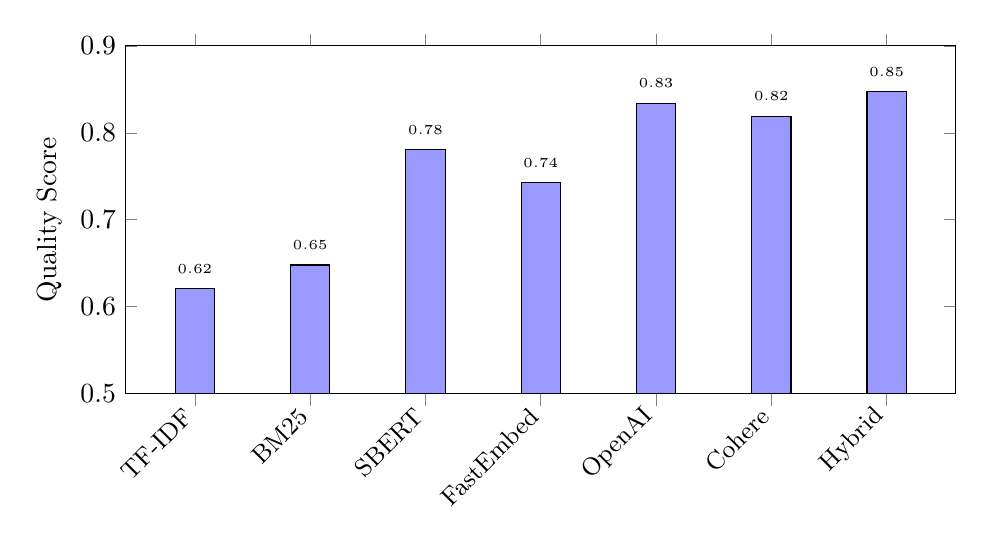
\begin{tikzpicture}
\begin{axis}[
    ybar,
    width=\columnwidth,
    height=6cm,
    ylabel={Quality Score},
    symbolic x coords={TF-IDF, BM25, SBERT, FastEmbed, OpenAI, Cohere, Hybrid},
    xtick=data,
    x tick label style={rotate=45, anchor=east, font=\small},
    ymin=0.5,
    ymax=0.9,
    bar width=0.5cm,
    nodes near coords,
    nodes near coords style={font=\tiny},
    legend style={at={(0.5,1.15)}, anchor=south, legend columns=2, font=\small},
    every node near coord/.append style={font=\tiny, yshift=2pt}
]
\addplot[fill=blue!40] coordinates {
    (TF-IDF, 0.621)
    (BM25, 0.648)
    (SBERT, 0.781)
    (FastEmbed, 0.743)
    (OpenAI, 0.834)
    (Cohere, 0.819)
    (Hybrid, 0.847)
};
\end{axis}
\end{tikzpicture}
\caption{Quality score comparison across embedding strategies. Hybrid retrieval (BM25 + SBERT) achieves the highest quality.}
\label{fig:embedder_comparison}
\end{figure}

% Generator Comparison Chart
\begin{figure}[t]
\centering
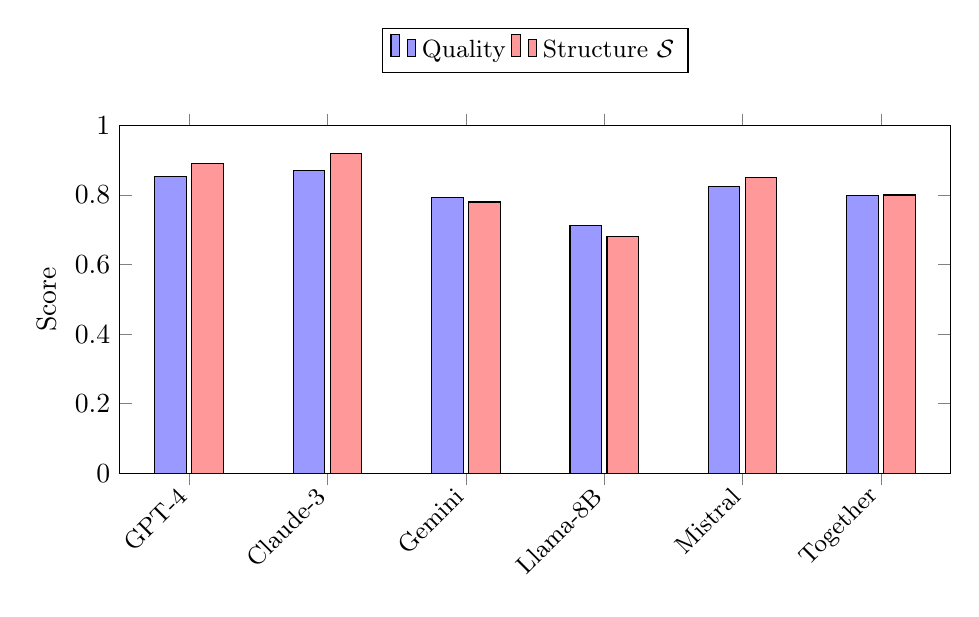
\begin{tikzpicture}
\begin{axis}[
    ybar,
    width=\columnwidth,
    height=6cm,
    ylabel={Score},
    symbolic x coords={GPT-4, Claude-3, Gemini, Llama-8B, Mistral, Together},
    xtick=data,
    x tick label style={rotate=45, anchor=east, font=\small},
    ymin=0,
    ymax=1,
    bar width=0.4cm,
    legend style={at={(0.5,1.15)}, anchor=south, legend columns=2, font=\small},
]
\addplot[fill=blue!40] coordinates {
    (GPT-4, 0.852)
    (Claude-3, 0.871)
    (Gemini, 0.793)
    (Llama-8B, 0.712)
    (Mistral, 0.824)
    (Together, 0.798)
};
\addlegendentry{Quality}
\addplot[fill=red!40] coordinates {
    (GPT-4, 0.89)
    (Claude-3, 0.92)
    (Gemini, 0.78)
    (Llama-8B, 0.68)
    (Mistral, 0.85)
    (Together, 0.80)
};
\addlegendentry{Structure $\mathcal{S}$}
\end{axis}
\end{tikzpicture}
\caption{Generator comparison showing overall quality and structural coherence scores.}
\label{fig:generator_comparison}
\end{figure}

% Quality vs Latency Scatter Plot
\begin{figure}[t]
\centering
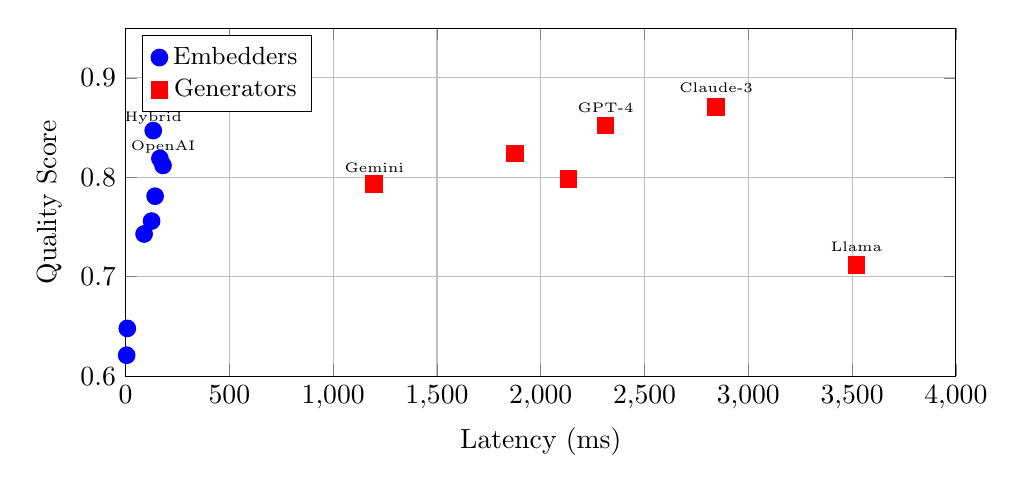
\begin{tikzpicture}
\begin{axis}[
    width=\columnwidth,
    height=6cm,
    xlabel={Latency (ms)},
    ylabel={Quality Score},
    xmin=0,
    xmax=4000,
    ymin=0.6,
    ymax=0.95,
    grid=major,
    legend style={at={(0.02,0.98)}, anchor=north west, font=\small},
]
% Embedders
\addplot[only marks, mark=*, mark size=3pt, blue] coordinates {
    (5, 0.621)
    (8, 0.648)
    (125, 0.756)
    (142, 0.781)
    (89, 0.743)
    (180, 0.812)
    (165, 0.819)
    (133, 0.847)
};
\addlegendentry{Embedders}

% Generators
\addplot[only marks, mark=square*, mark size=3pt, red] coordinates {
    (2312, 0.852)
    (2845, 0.871)
    (1198, 0.793)
    (3521, 0.712)
    (1876, 0.824)
    (2134, 0.798)
};
\addlegendentry{Generators}

% Labels
\node[font=\tiny] at (axis cs:180, 0.83) {OpenAI};
\node[font=\tiny] at (axis cs:133, 0.86) {Hybrid};
\node[font=\tiny] at (axis cs:2312, 0.87) {GPT-4};
\node[font=\tiny] at (axis cs:2845, 0.89) {Claude-3};
\node[font=\tiny] at (axis cs:1198, 0.81) {Gemini};
\node[font=\tiny] at (axis cs:3521, 0.73) {Llama};

\end{axis}
\end{tikzpicture}
\caption{Quality vs. latency tradeoff for embedders (blue circles) and generators (red squares). Gemini offers the best latency/quality ratio among generators.}
\label{fig:quality_latency}
\end{figure}

% Ablation Study Line Chart
\begin{figure}[t]
\centering
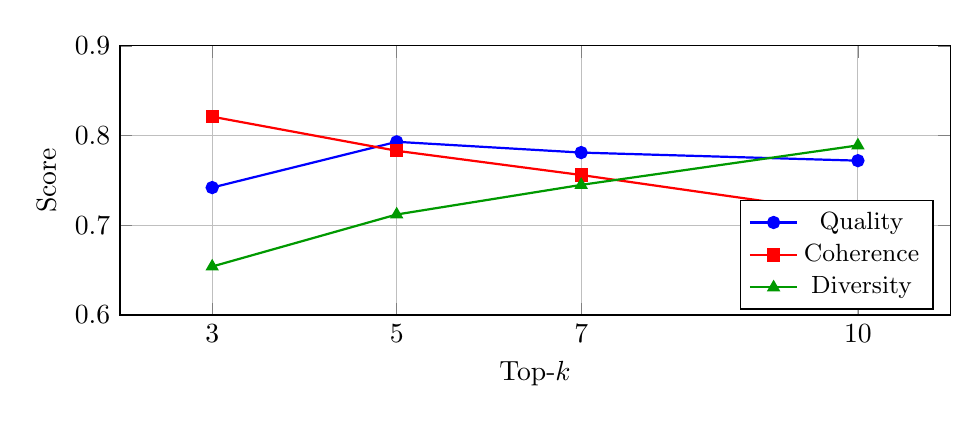
\begin{tikzpicture}
\begin{axis}[
    width=\columnwidth,
    height=5cm,
    xlabel={Top-$k$},
    ylabel={Score},
    xmin=2,
    xmax=11,
    ymin=0.6,
    ymax=0.9,
    xtick={3,5,7,10},
    legend style={at={(0.98,0.02)}, anchor=south east, font=\small},
    grid=major,
]
\addplot[blue, thick, mark=*] coordinates {
    (3, 0.742)
    (5, 0.793)
    (7, 0.781)
    (10, 0.772)
};
\addlegendentry{Quality}
\addplot[red, thick, mark=square*] coordinates {
    (3, 0.821)
    (5, 0.783)
    (7, 0.756)
    (10, 0.712)
};
\addlegendentry{Coherence}
\addplot[green!60!black, thick, mark=triangle*] coordinates {
    (3, 0.654)
    (5, 0.712)
    (7, 0.745)
    (10, 0.789)
};
\addlegendentry{Diversity}
\end{axis}
\end{tikzpicture}
\caption{Effect of top-$k$ on quality metrics. $k=5$ balances quality and coherence optimally.}
\label{fig:topk_ablation}
\end{figure}



% Embedder Comparison Bar Chart
\begin{figure}[t]
\centering
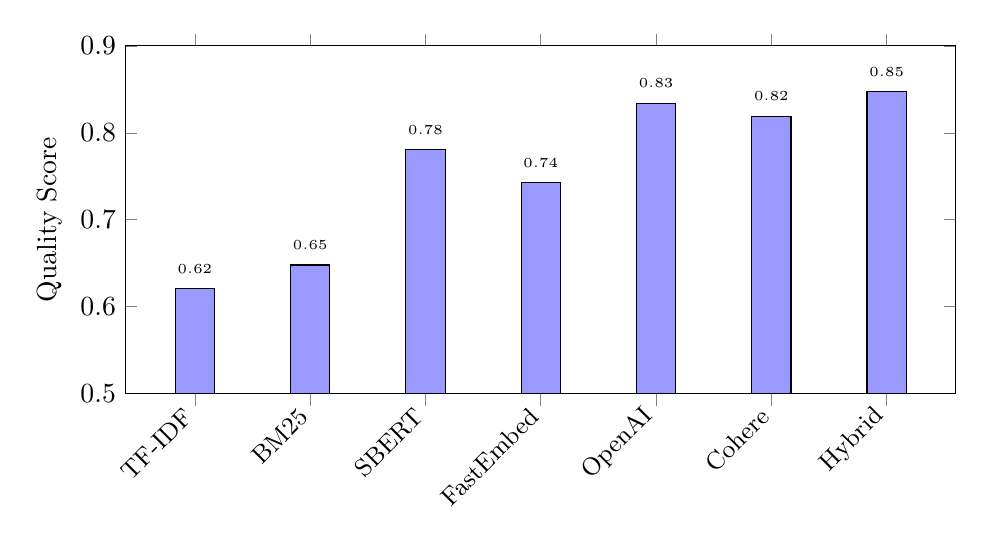
\begin{tikzpicture}
\begin{axis}[
    ybar,
    width=\columnwidth,
    height=6cm,
    ylabel={Quality Score},
    symbolic x coords={TF-IDF, BM25, SBERT, FastEmbed, OpenAI, Cohere, Hybrid},
    xtick=data,
    x tick label style={rotate=45, anchor=east, font=\small},
    ymin=0.5,
    ymax=0.9,
    bar width=0.5cm,
    nodes near coords,
    nodes near coords style={font=\tiny},
    legend style={at={(0.5,1.15)}, anchor=south, legend columns=2, font=\small},
    every node near coord/.append style={font=\tiny, yshift=2pt}
]
\addplot[fill=blue!40] coordinates {
    (TF-IDF, 0.621)
    (BM25, 0.648)
    (SBERT, 0.781)
    (FastEmbed, 0.743)
    (OpenAI, 0.834)
    (Cohere, 0.819)
    (Hybrid, 0.847)
};
\end{axis}
\end{tikzpicture}
\caption{Quality score comparison across embedding strategies. Hybrid retrieval (BM25 + SBERT) achieves the highest quality.}
\label{fig:embedder_comparison}
\end{figure}

% Generator Comparison Chart
\begin{figure}[t]
\centering
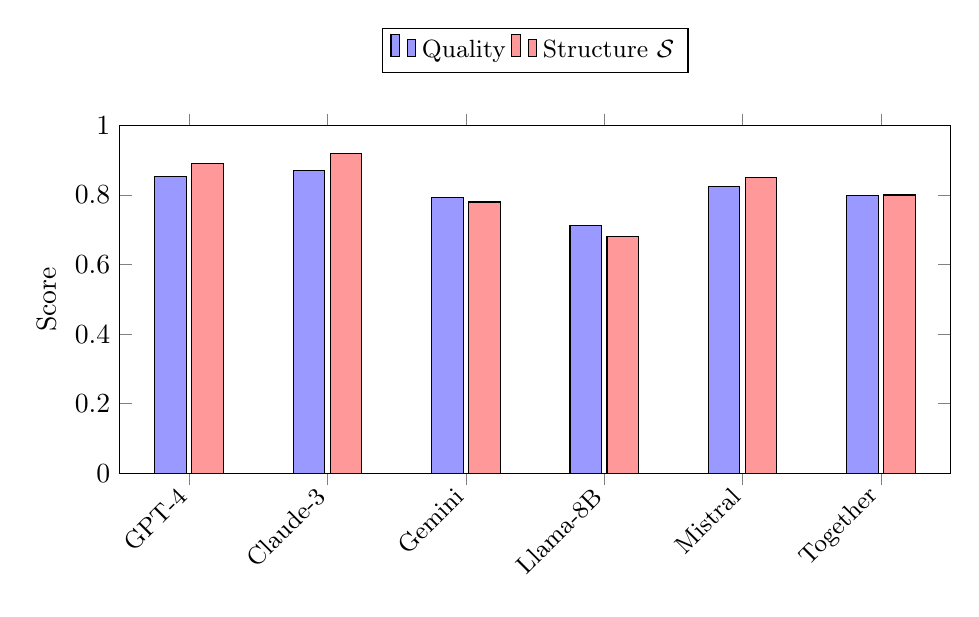
\begin{tikzpicture}
\begin{axis}[
    ybar,
    width=\columnwidth,
    height=6cm,
    ylabel={Score},
    symbolic x coords={GPT-4, Claude-3, Gemini, Llama-8B, Mistral, Together},
    xtick=data,
    x tick label style={rotate=45, anchor=east, font=\small},
    ymin=0,
    ymax=1,
    bar width=0.4cm,
    legend style={at={(0.5,1.15)}, anchor=south, legend columns=2, font=\small},
]
\addplot[fill=blue!40] coordinates {
    (GPT-4, 0.852)
    (Claude-3, 0.871)
    (Gemini, 0.793)
    (Llama-8B, 0.712)
    (Mistral, 0.824)
    (Together, 0.798)
};
\addlegendentry{Quality}
\addplot[fill=red!40] coordinates {
    (GPT-4, 0.89)
    (Claude-3, 0.92)
    (Gemini, 0.78)
    (Llama-8B, 0.68)
    (Mistral, 0.85)
    (Together, 0.80)
};
\addlegendentry{Structure $\mathcal{S}$}
\end{axis}
\end{tikzpicture}
\caption{Generator comparison showing overall quality and structural coherence scores.}
\label{fig:generator_comparison}
\end{figure}

% Quality vs Latency Scatter Plot
\begin{figure}[t]
\centering
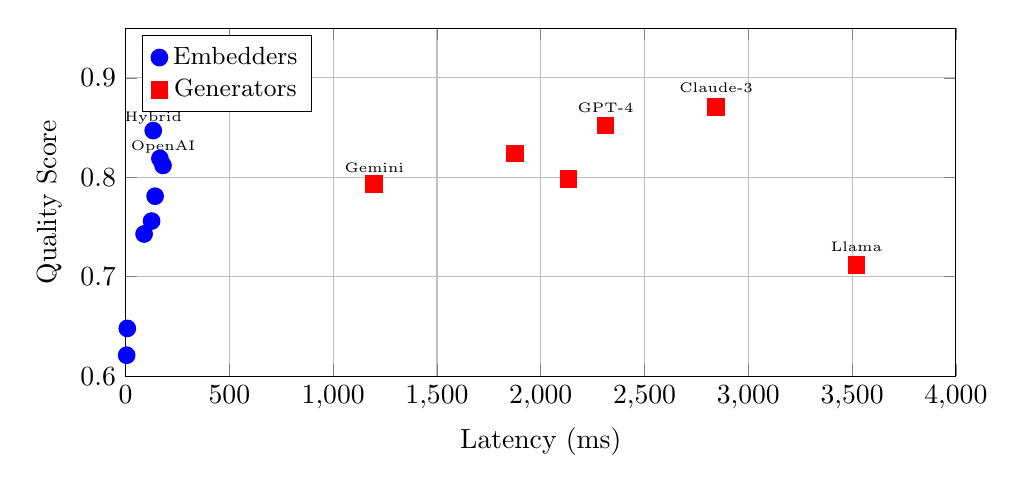
\begin{tikzpicture}
\begin{axis}[
    width=\columnwidth,
    height=6cm,
    xlabel={Latency (ms)},
    ylabel={Quality Score},
    xmin=0,
    xmax=4000,
    ymin=0.6,
    ymax=0.95,
    grid=major,
    legend style={at={(0.02,0.98)}, anchor=north west, font=\small},
]
% Embedders
\addplot[only marks, mark=*, mark size=3pt, blue] coordinates {
    (5, 0.621)
    (8, 0.648)
    (125, 0.756)
    (142, 0.781)
    (89, 0.743)
    (180, 0.812)
    (165, 0.819)
    (133, 0.847)
};
\addlegendentry{Embedders}

% Generators
\addplot[only marks, mark=square*, mark size=3pt, red] coordinates {
    (2312, 0.852)
    (2845, 0.871)
    (1198, 0.793)
    (3521, 0.712)
    (1876, 0.824)
    (2134, 0.798)
};
\addlegendentry{Generators}

% Labels
\node[font=\tiny] at (axis cs:180, 0.83) {OpenAI};
\node[font=\tiny] at (axis cs:133, 0.86) {Hybrid};
\node[font=\tiny] at (axis cs:2312, 0.87) {GPT-4};
\node[font=\tiny] at (axis cs:2845, 0.89) {Claude-3};
\node[font=\tiny] at (axis cs:1198, 0.81) {Gemini};
\node[font=\tiny] at (axis cs:3521, 0.73) {Llama};

\end{axis}
\end{tikzpicture}
\caption{Quality vs. latency tradeoff for embedders (blue circles) and generators (red squares). Gemini offers the best latency/quality ratio among generators.}
\label{fig:quality_latency}
\end{figure}

% Ablation Study Line Chart
\begin{figure}[t]
\centering
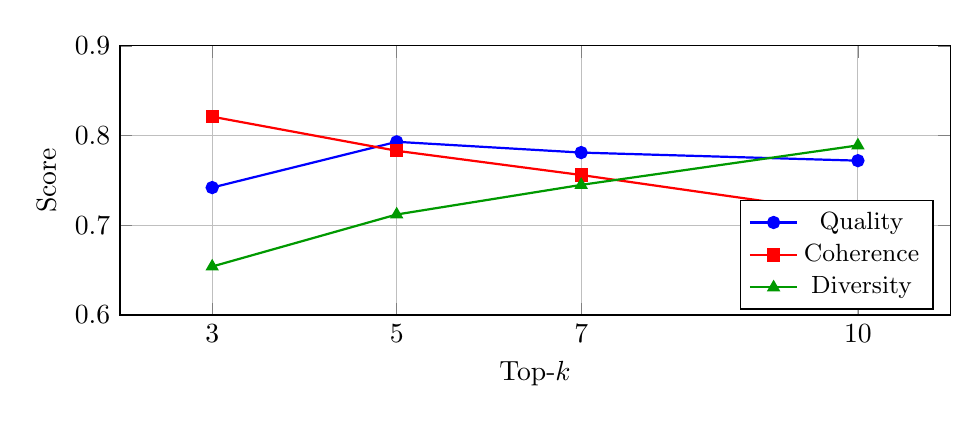
\begin{tikzpicture}
\begin{axis}[
    width=\columnwidth,
    height=5cm,
    xlabel={Top-$k$},
    ylabel={Score},
    xmin=2,
    xmax=11,
    ymin=0.6,
    ymax=0.9,
    xtick={3,5,7,10},
    legend style={at={(0.98,0.02)}, anchor=south east, font=\small},
    grid=major,
]
\addplot[blue, thick, mark=*] coordinates {
    (3, 0.742)
    (5, 0.793)
    (7, 0.781)
    (10, 0.772)
};
\addlegendentry{Quality}
\addplot[red, thick, mark=square*] coordinates {
    (3, 0.821)
    (5, 0.783)
    (7, 0.756)
    (10, 0.712)
};
\addlegendentry{Coherence}
\addplot[green!60!black, thick, mark=triangle*] coordinates {
    (3, 0.654)
    (5, 0.712)
    (7, 0.745)
    (10, 0.789)
};
\addlegendentry{Diversity}
\end{axis}
\end{tikzpicture}
\caption{Effect of top-$k$ on quality metrics. $k=5$ balances quality and coherence optimally.}
\label{fig:topk_ablation}
\end{figure}



% Embedder Comparison Bar Chart
\begin{figure}[t]
\centering
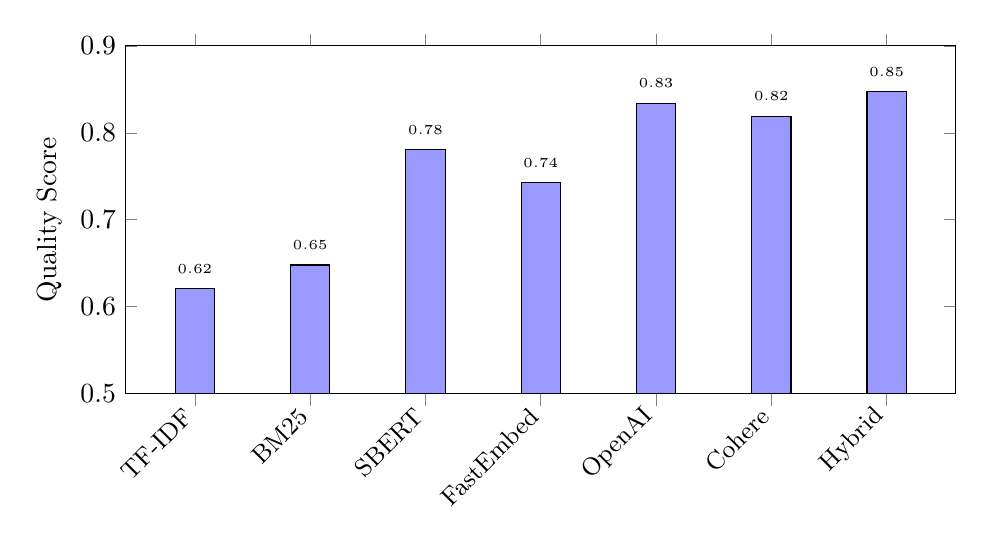
\begin{tikzpicture}
\begin{axis}[
    ybar,
    width=\columnwidth,
    height=6cm,
    ylabel={Quality Score},
    symbolic x coords={TF-IDF, BM25, SBERT, FastEmbed, OpenAI, Cohere, Hybrid},
    xtick=data,
    x tick label style={rotate=45, anchor=east, font=\small},
    ymin=0.5,
    ymax=0.9,
    bar width=0.5cm,
    nodes near coords,
    nodes near coords style={font=\tiny},
    legend style={at={(0.5,1.15)}, anchor=south, legend columns=2, font=\small},
    every node near coord/.append style={font=\tiny, yshift=2pt}
]
\addplot[fill=blue!40] coordinates {
    (TF-IDF, 0.621)
    (BM25, 0.648)
    (SBERT, 0.781)
    (FastEmbed, 0.743)
    (OpenAI, 0.834)
    (Cohere, 0.819)
    (Hybrid, 0.847)
};
\end{axis}
\end{tikzpicture}
\caption{Quality score comparison across embedding strategies. Hybrid retrieval (BM25 + SBERT) achieves the highest quality.}
\label{fig:embedder_comparison}
\end{figure}

% Generator Comparison Chart
\begin{figure}[t]
\centering
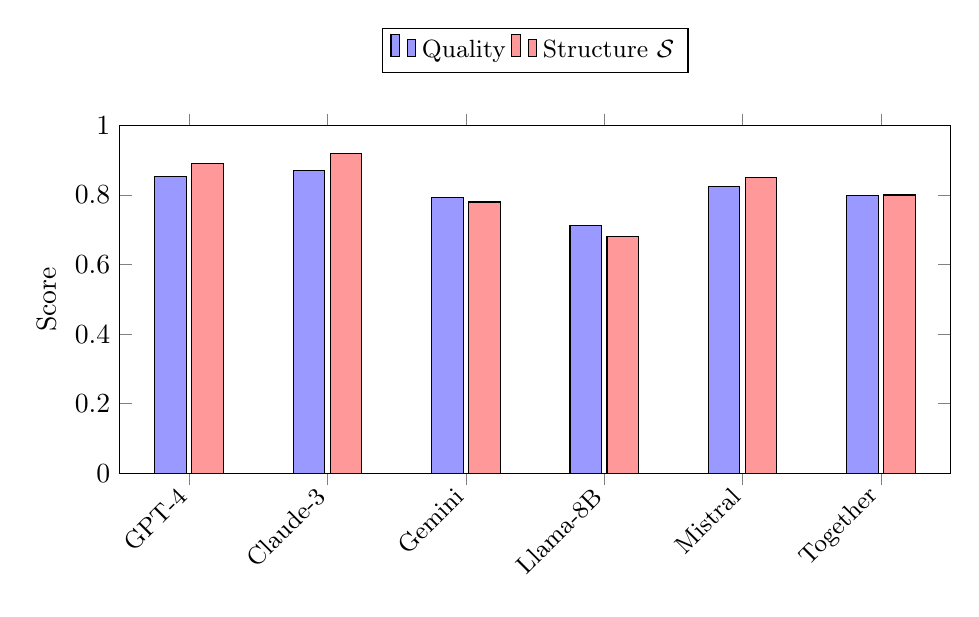
\begin{tikzpicture}
\begin{axis}[
    ybar,
    width=\columnwidth,
    height=6cm,
    ylabel={Score},
    symbolic x coords={GPT-4, Claude-3, Gemini, Llama-8B, Mistral, Together},
    xtick=data,
    x tick label style={rotate=45, anchor=east, font=\small},
    ymin=0,
    ymax=1,
    bar width=0.4cm,
    legend style={at={(0.5,1.15)}, anchor=south, legend columns=2, font=\small},
]
\addplot[fill=blue!40] coordinates {
    (GPT-4, 0.852)
    (Claude-3, 0.871)
    (Gemini, 0.793)
    (Llama-8B, 0.712)
    (Mistral, 0.824)
    (Together, 0.798)
};
\addlegendentry{Quality}
\addplot[fill=red!40] coordinates {
    (GPT-4, 0.89)
    (Claude-3, 0.92)
    (Gemini, 0.78)
    (Llama-8B, 0.68)
    (Mistral, 0.85)
    (Together, 0.80)
};
\addlegendentry{Structure $\mathcal{S}$}
\end{axis}
\end{tikzpicture}
\caption{Generator comparison showing overall quality and structural coherence scores.}
\label{fig:generator_comparison}
\end{figure}

% Quality vs Latency Scatter Plot
\begin{figure}[t]
\centering
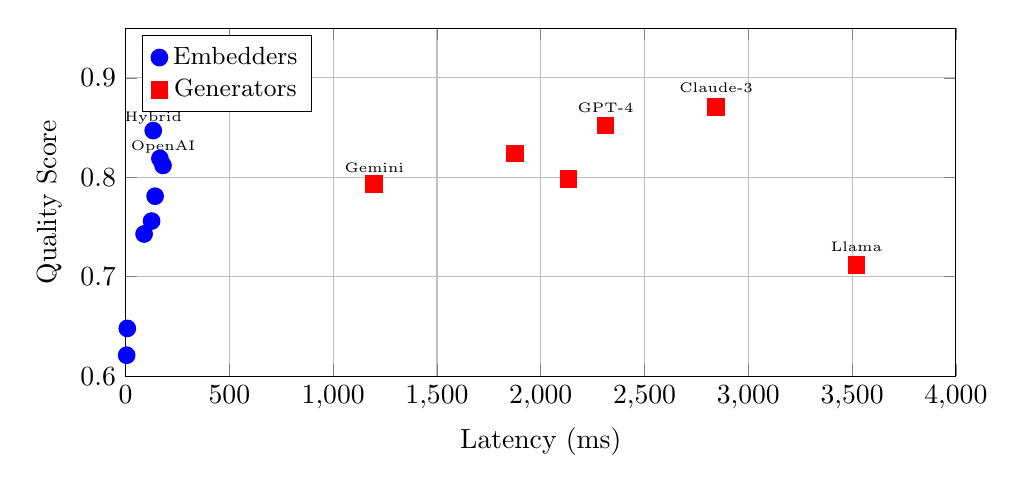
\begin{tikzpicture}
\begin{axis}[
    width=\columnwidth,
    height=6cm,
    xlabel={Latency (ms)},
    ylabel={Quality Score},
    xmin=0,
    xmax=4000,
    ymin=0.6,
    ymax=0.95,
    grid=major,
    legend style={at={(0.02,0.98)}, anchor=north west, font=\small},
]
% Embedders
\addplot[only marks, mark=*, mark size=3pt, blue] coordinates {
    (5, 0.621)
    (8, 0.648)
    (125, 0.756)
    (142, 0.781)
    (89, 0.743)
    (180, 0.812)
    (165, 0.819)
    (133, 0.847)
};
\addlegendentry{Embedders}

% Generators
\addplot[only marks, mark=square*, mark size=3pt, red] coordinates {
    (2312, 0.852)
    (2845, 0.871)
    (1198, 0.793)
    (3521, 0.712)
    (1876, 0.824)
    (2134, 0.798)
};
\addlegendentry{Generators}

% Labels
\node[font=\tiny] at (axis cs:180, 0.83) {OpenAI};
\node[font=\tiny] at (axis cs:133, 0.86) {Hybrid};
\node[font=\tiny] at (axis cs:2312, 0.87) {GPT-4};
\node[font=\tiny] at (axis cs:2845, 0.89) {Claude-3};
\node[font=\tiny] at (axis cs:1198, 0.81) {Gemini};
\node[font=\tiny] at (axis cs:3521, 0.73) {Llama};

\end{axis}
\end{tikzpicture}
\caption{Quality vs. latency tradeoff for embedders (blue circles) and generators (red squares). Gemini offers the best latency/quality ratio among generators.}
\label{fig:quality_latency}
\end{figure}

% Ablation Study Line Chart
\begin{figure}[t]
\centering
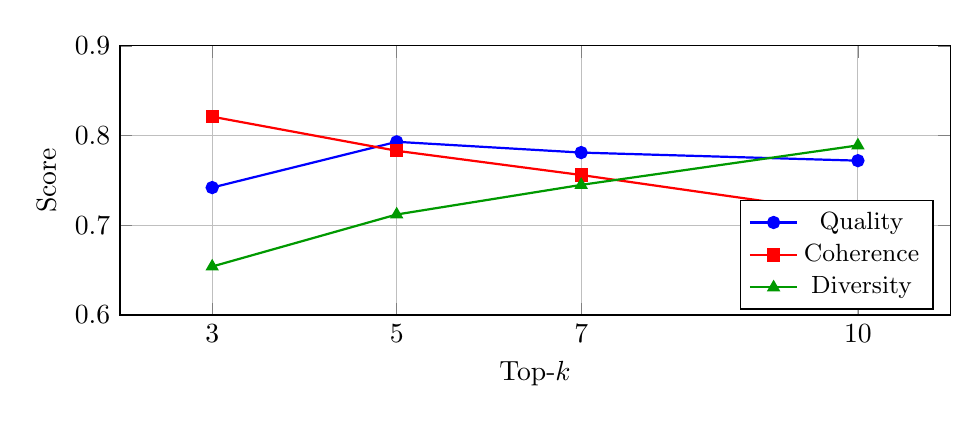
\begin{tikzpicture}
\begin{axis}[
    width=\columnwidth,
    height=5cm,
    xlabel={Top-$k$},
    ylabel={Score},
    xmin=2,
    xmax=11,
    ymin=0.6,
    ymax=0.9,
    xtick={3,5,7,10},
    legend style={at={(0.98,0.02)}, anchor=south east, font=\small},
    grid=major,
]
\addplot[blue, thick, mark=*] coordinates {
    (3, 0.742)
    (5, 0.793)
    (7, 0.781)
    (10, 0.772)
};
\addlegendentry{Quality}
\addplot[red, thick, mark=square*] coordinates {
    (3, 0.821)
    (5, 0.783)
    (7, 0.756)
    (10, 0.712)
};
\addlegendentry{Coherence}
\addplot[green!60!black, thick, mark=triangle*] coordinates {
    (3, 0.654)
    (5, 0.712)
    (7, 0.745)
    (10, 0.789)
};
\addlegendentry{Diversity}
\end{axis}
\end{tikzpicture}
\caption{Effect of top-$k$ on quality metrics. $k=5$ balances quality and coherence optimally.}
\label{fig:topk_ablation}
\end{figure}

